\chapter {Kế hoạch triển khai}
Với những mục tiêu đã đề ra ở mục \ref{sec:muctieu}, đề tài được thực hiện qua các giai đoạn như sau:

\begin{itemize}
    \item \textbf{Giai đoạn 1:} Tìm kiếm và thu thập các thông tin về sản phẩm thời trang để thiết kế ra các hoạt động mà Chatbot có thể hỗ trợ.
    \item \textbf{Giai đoạn 2:} Khảo sát và thu thập các thông tin từ người dùng để thiết kế ra các ý định của người dùng.
    \item \textbf{Giai đoạn 3:} Định nghĩa cách kiểm thử và đánh giá hệ thống.
    \item \textbf{Giai đoạn 4:} Xây dựng bộ mô phỏng người dùng và lỗi.
    \item \textbf{Giai đoạn 5:} Xây dựng bộ quản lý hội thoại.
    \item \textbf{Giai đoạn 6:} Tích hợp các thành phần còn lại.
    \item \textbf{Giai đoạn 7:} Tiến hành kiểm thử và đánh giá hệ thống.
\end{itemize}

Thời gian cụ thể thực hiện được mô tả như sau:

\begin{center}
    \begin{figure}[h!]
        \begin{center}
         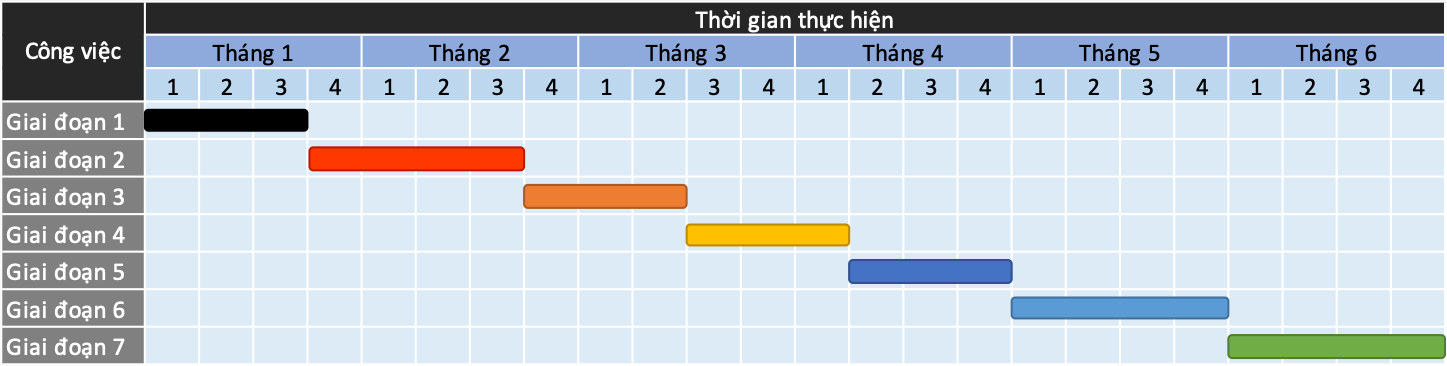
\includegraphics[scale=0.63]{chapter4.5/img/timeline.png}
        \end{center}
        \caption{Thời gian thực hiện đề tài}
    \end{figure}
\end{center}